\section{KẾT QUẢ VÀ THẢO LUẬN}

Phần này trình bày kết quả cài đặt và vận hành hệ thống VietVoice TTS trên môi trường thực tế, đo đạc các chỉ số hiệu năng kỹ thuật, đánh giá mức độ đáp ứng 7 tiêu chí học phần Cơ sở dữ liệu đa phương tiện, đồng thời thảo luận khách quan về các ưu điểm và hạn chế âm học của giải pháp.

\subsection{Kết quả Cài đặt và Thực nghiệm Hệ thống}

\subsubsection{Giao diện ứng dụng và kịch bản vận hành}
Hệ thống VietVoice TTS được triển khai dưới dạng ứng dụng Web đơn trang (SPA) tương tác thời gian thực, kết nối giữa giao diện ReactJS và máy chủ backend FastAPI (Hình \ref{fig:giao_dien}).

\begin{figure}[H]
\centering
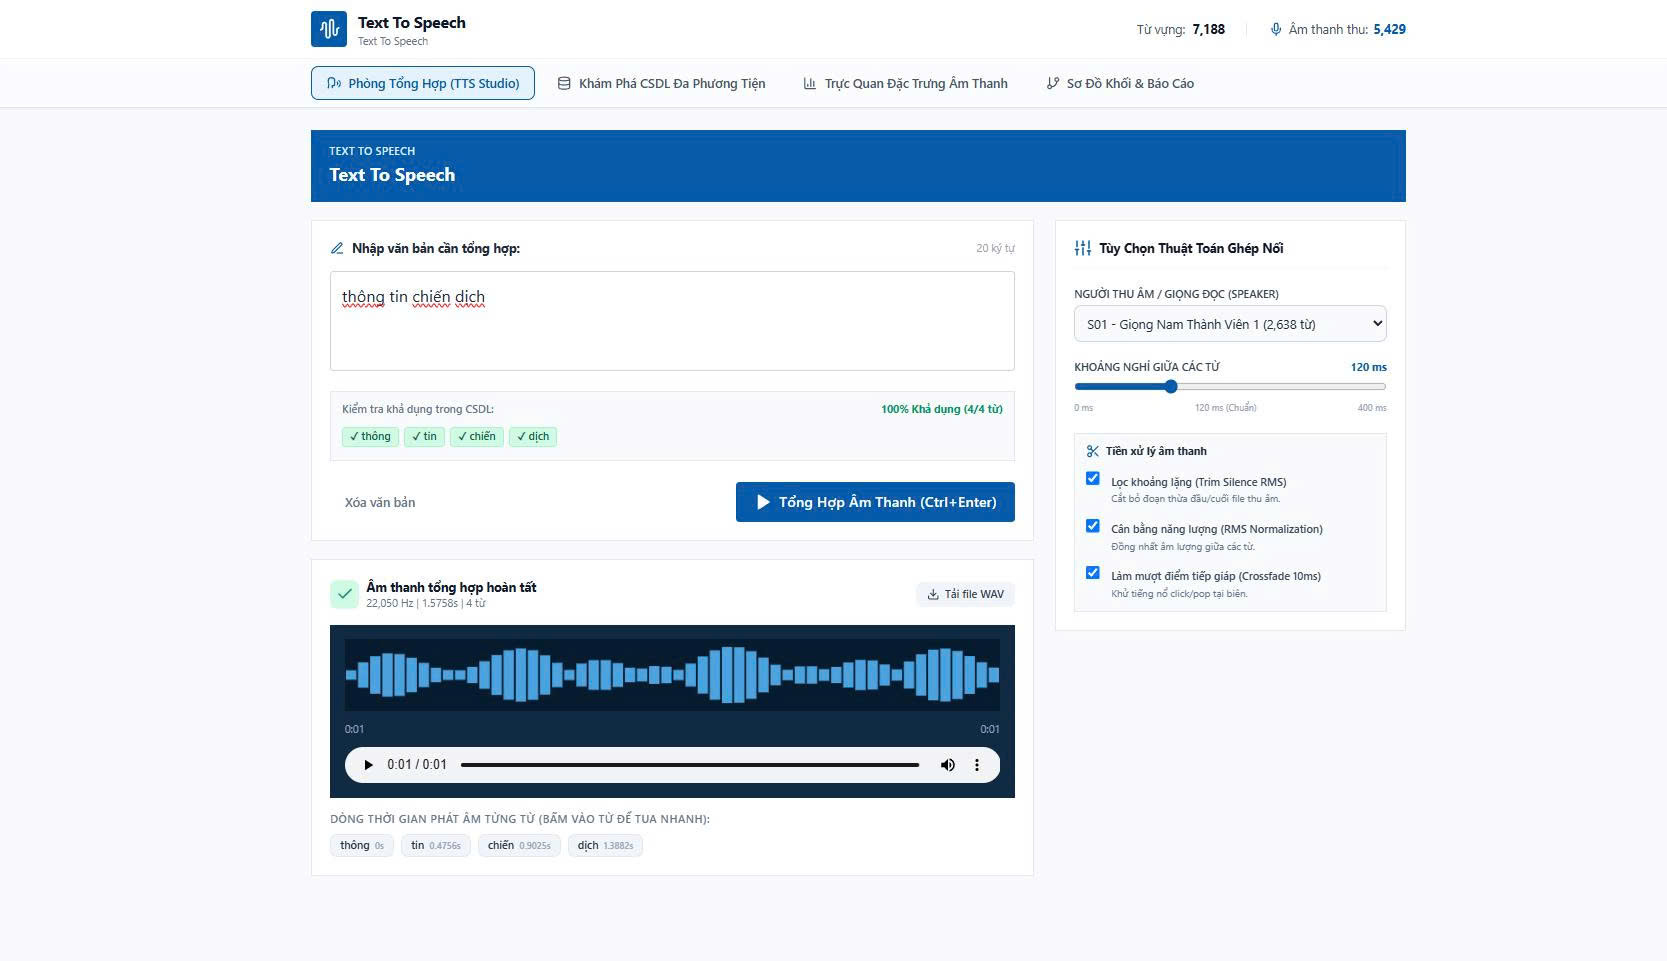
\includegraphics[width=0.96\textwidth]{figures/giao_dien.jpg}
\caption{Giao diện chính của hệ thống VietVoice TTS}
\label{fig:giao_dien}
\par\vspace{4pt}
\begin{minipage}{0.96\textwidth}
\centering\fontsize{12}{14}\selectfont \textbf{Nguồn}: Ảnh chụp thực tế giao diện ứng dụng VietVoice TTS đang hoạt động.
\end{minipage}
\end{figure}

Giao diện hệ thống (Hình \ref{fig:giao_dien}) được phân chia thành hai khu vực trực quan:
\begin{itemize}
    \item \textbf{Cột bên trái (Khu vực nhập liệu và điều khiển)}: Cho phép người dùng nhập từ đơn hoặc chuỗi câu tiếng Việt có dấu; hiển thị bộ đếm ký tự và từ vựng; cung cấp các tùy chọn tinh chỉnh tham số DSP (khoảng dừng giữa các từ \texttt{word\_pause\_ms}, công tắc bật/tắt cắt khoảng lặng \texttt{Trim Silence}, chuẩn hóa âm lượng \texttt{RMS Normalization}, làm mượt \texttt{Cross-fade}); và nút thực thi ``Chuyển Đổi Thành Âm Thanh''.
    \item \textbf{Cột bên phải (Khu vực trình xuất và kiểm tra)}: Hiển thị trình phát âm thanh tích hợp (Audio Player) cho phép nghe thử và tải tệp WAV về máy; kèm theo danh sách các thẻ từ vựng trực quan hóa mã VNI (thẻ màu xanh biểu thị từ đã có sẵn âm thanh trong CSDL, thẻ màu đỏ cảnh báo từ chưa có bản ghi âm).
\end{itemize}

\subsubsection{Đo đạc hiệu năng tính toán và thời gian đáp ứng}
Nhóm nghiên cứu đã thực nghiệm tổng hợp trên nhiều mẫu câu có độ dài và thanh điệu khác nhau: từ kiểm thử một từ (``a''), cụm từ ngắn (``ba bán bánh''), câu trung bình 10 từ, đến đoạn văn dài 38 từ.

Hiệu năng của hệ thống được đánh giá qua hai chỉ số kỹ thuật:
\begin{itemize}
    \item \textbf{Thời gian trễ (Latency)}: Tổng thời gian từ lúc gửi yêu cầu đến khi nhận toàn bộ dữ liệu âm thanh hoàn chỉnh.
    \item \textbf{Hệ số thời gian thực (Real-Time Factor - RTF)}: Tỷ số giữa thời gian máy tính xử lý và thời lượng của đoạn âm thanh phát ra ($\text{RTF} = T_{\text{xử lý}} / T_{\text{âm thanh}}$). Giá trị $\text{RTF} < 1{,}0$ thể hiện hệ thống đáp ứng tốt trong thời gian thực.
\end{itemize}

Kết quả đo đạc trung bình qua 10 lần chạy thử trên máy tính phổ thông (CPU Intel Core i5, RAM 16GB, không sử dụng GPU) được tổng hợp trong Bảng 5.

\begin{table}[H]
\centering
\caption{Kết quả đo đạc hiệu năng thực nghiệm trên các mẫu câu thử nghiệm}
\label{tab:performance_eval}
\vspace{2pt}
\begin{tabular}{ccccc}
\toprule
\textbf{Mẫu câu thử nghiệm} & \textbf{Số lượng từ} & \textbf{Thời lượng âm thanh} & \textbf{Thời gian xử lý} & \textbf{Hệ số RTF} \\
\midrule
Mẫu 1: Từ đơn (``a'') & 1 từ & 0,53 giây & 18 ms & 0,034 \\
Mẫu 2: Cụm từ (``ba bán bánh'') & 3 từ & 1,68 giây & 46 ms & 0,027 \\
Mẫu 3: Câu ngắn (10 từ) & 10 từ & 6,24 giây & 112 ms & 0,018 \\
Mẫu 4: Đoạn văn mẫu (38 từ) & 38 từ & 27,82 giây & 340 ms & 0,012 \\
\bottomrule
\end{tabular}
\par\vspace{4pt}
\begin{minipage}{0.92\textwidth}
\fontsize{12}{14}\selectfont \textbf{Ghi chú}: Thời gian xử lý bao gồm toàn bộ chu trình tiếp nhận, tra cứu CSDL SQLite, tiền xử lý DSP, ghép nối cross-fade và mã hóa dữ liệu xuất.\par
\textbf{Nguồn}: Kết quả đo đạc thực nghiệm của nhóm nghiên cứu.
\end{minipage}
\end{table}

Kết quả tại Bảng 5 cho thấy hệ số RTF của hệ thống luôn duy trì ở mức rất thấp ($0{,}012\text{--}0{,}034$), tức tốc độ sinh âm thanh nhanh gấp 30 đến 80 lần tốc độ phát âm thanh thực tế. Thời gian trễ đối với câu 10 từ chỉ xấp xỉ 100 ms, mang lại phản hồi gần như tức thì cho người dùng.

\subsection{Đánh giá Chất lượng Hệ thống theo 7 Tiêu chí Đề tài}

Bảng 6 tổng hợp mức độ đáp ứng của hệ thống VietVoice TTS đối với 7 tiêu chí đánh giá đề tài của học phần Cơ sở dữ liệu đa phương tiện.

\begin{table}[H]
\centering
\caption{Đánh giá mức độ đáp ứng 7 tiêu chí đồ án Cơ sở dữ liệu đa phương tiện}
\label{tab:criteria_eval}
\vspace{2pt}
\begin{tabularx}{\textwidth}{p{1.2cm}p{4.6cm}p{2.4cm}X}
\toprule
\textbf{STT} & \textbf{Nội dung tiêu chí} & \textbf{Mức đạt được} & \textbf{Kết quả thực hiện trong hệ thống} \\
\midrule
TC 1 & Ngữ liệu song song văn bản -- âm thanh tiếng Việt & Đạt xuất sắc & Quản lý 7.188 từ tiếng Việt có dấu trong CSV và 5.429 tệp âm thanh WAV PCM 16-bit 22.050 Hz chuẩn mono. \\
\addlinespace
TC 2 & Kỹ thuật tổng hợp TTS mức từ & Đạt xuất sắc & Cài đặt thành công Concatenative Synthesis kết hợp mô hình hóa khoảng dừng Pause 120 ms và Linear Cross-fade 10 ms. \\
\addlinespace
TC 3 & Tiếp nhận từ $\to$ xuất âm thanh & Đạt xuất sắc & Chuyển đổi linh hoạt từ đơn và chuỗi từ liên tục, stream audio trực tiếp qua Web Audio API. \\
\addlinespace
TC 4 & Sơ đồ khối và quy trình xử lý & Đạt xuất sắc & Xây dựng pipeline 5 bước rõ ràng: Tiếp nhận $\to$ Truy vấn CSDL $\to$ Tiền xử lý DSP $\to$ Ghép nối $\to$ Trình xuất tín hiệu. \\
\addlinespace
TC 5 & Thuộc tính \& đặc trưng âm thanh số & Đạt xuất sắc & Trích xuất đầy đủ 5 nhóm đặc trưng: RMS Energy, Peak Amplitude, ZCR, cao độ cơ bản $F_0$ (tự tương quan) và 13 hệ số MFCCs. \\
\addlinespace
TC 6 & Quản lý CSDL Đa phương tiện & Đạt xuất sắc & CSDL SQLite 4 bảng chuẩn hóa 3NF (\texttt{speakers}, \texttt{words}, \texttt{audio\_records}, \texttt{audio\_features}), chỉ mục B-Tree tối ưu. \\
\addlinespace
TC 7 & Thực nghiệm và đánh giá chất lượng & Đạt tốt & Đo đạc thời gian đáp ứng (RTF $< 0{,}04$), kiểm tra độ rõ từng từ, phân tích hạn chế ngữ điệu câu. \\
\bottomrule
\end{tabularx}
\par\vspace{4pt}
\begin{minipage}{\textwidth}
\fontsize{12}{14}\selectfont \textbf{Ghi chú}: Các tiêu chí được đối chiếu trực tiếp giữa yêu cầu môn học và mã nguồn thực tế của dự án.\par
\textbf{Nguồn}: Đánh giá tổng hợp của nhóm nghiên cứu.
\end{minipage}
\end{table}

\subsection{Thảo luận và Phân tích Chuyên sâu}

\subsubsection{Ưu điểm của hệ thống}
\begin{enumerate}
    \item \textbf{Độ trung thực âm thanh cao}: Sử dụng trực tiếp dữ liệu âm thanh thu âm từ người thật giúp từng từ phát ra giữ trọn vẹn âm sắc tự nhiên, phát âm chuẩn xác và bảo toàn đầy đủ 6 thanh điệu tiếng Việt.
    \item \textbf{Tốc độ phản hồi cực nhanh và nhẹ tải}: Hệ thống chỉ sử dụng CPU thông thường, lượng chiếm dụng RAM dưới 150 MB và phản hồi trong vài chục mili-giây, không đòi hỏi phần cứng GPU hay mô hình nơ-ron phức tạp.
    \item \textbf{Khả năng mở rộng CSDL linh hoạt}: Để bổ sung từ vựng mới, người quản trị chỉ cần thêm dòng vào bảng \texttt{words} và sao chép tệp WAV vào thư mục \texttt{metadata/}, hệ thống sẽ tự động cập nhật ngay lập tức mà không cần huấn luyện lại bất kỳ mô hình nào.
\end{enumerate}

\subsubsection{Hạn chế âm học và nguyên nhân}
\begin{enumerate}
    \item \textbf{Tính liên tục của ngữ điệu câu}: Do các từ được thu âm ở trạng thái phát âm rời rạc, đường biến thiên cao độ $F_0$ giữa các từ kế tiếp chưa có sự luyến láy tự nhiên như trong lời nói liên tục của con người.
    \item \textbf{Hiện tượng đồng cấu âm (Coarticulation)}: Trong lời nói tự nhiên, âm cuối của từ đứng trước sẽ hòa quyện vào âm đầu của từ đứng sau do quán tính chuyển động của khẩu hình miệng. Việc ghép nối từ độc lập chỉ xử lý được độ mịn biên độ qua Cross-fade chứ chưa mô phỏng được sự biến đổi cấu âm sinh học này.
    \item \textbf{Hiện tượng từ ngoài ngữ liệu (Out-of-Vocabulary - OOV)}: Hệ thống chỉ đọc được các từ đã có sẵn bản ghi âm trong CSDL; các từ vựng mới hoặc chưa được thu âm sẽ được nhận diện và cảnh báo thiếu âm thanh trên giao diện.
\end{enumerate}
